%%%%%%%%%%%%%%%%%%%%%%%%%%%%%%%%%%%%%%%%%
\title{Tiểu luận về thương mại điện tử - Nhóm 5 - Chuyên nghiệp trong công nghệ}
%----------------------------------------------------------------------------------------
%	CONFIGURATIONS
%----------------------------------------------------------------------------------------

\documentclass[12pt]{article}
\usepackage[T5]{fontenc}
\usepackage[utf8]{inputenc}
\usepackage[vietnamese,english]{babel}
\usepackage{amsmath}
\usepackage{graphicx}
\usepackage[colorinlistoftodos]{todonotes}
\usepackage{listings}
\usepackage{hyperref}
\usepackage{multicol}
\hypersetup{
    colorlinks=true,
    linkcolor=blue,
    filecolor=magenta,      
    urlcolor=cyan,
}
\setlength{\parindent}{1em}
\setlength{\parskip}{1em}
\renewcommand{\baselinestretch}{1.5}
\addto\captionsenglish{
  \renewcommand{\contentsname}
    {Mục Lục}
}


\begin{document}
\begin{titlepage}

\newcommand{\HRule}{\rule{\linewidth}{0.5mm}}
\center
 
%----------------------------------------------------------------------------------------
%	HEADING
%----------------------------------------------------------------------------------------

\textsc{\LARGE ĐẠI HỌC CÔNG NGHỆ - ĐHQGHN}\\[1.5cm]
\textsc{\Large Môn học: Chuyên Nghiệp Trong Công Nghệ}\\[0.5cm]
\textsc{\large Bài tiểu luận Nhóm 5 }\\[0.5cm]

%----------------------------------------------------------------------------------------
%	TITLE
%----------------------------------------------------------------------------------------

\HRule \\[0.4cm]
{ \huge \bfseries THƯƠNG MẠI ĐIỆN TỬ}\\[0.4cm] % Title of your document
\HRule \\[1.5cm]
 
%----------------------------------------------------------------------------------------
%	AUTHOR
%----------------------------------------------------------------------------------------

\begin{minipage}{1.2\textwidth}
\begin{multicols}{2}
\begin{itemize}
    \item Nguyễn Văn Huy
    \item Ngô Văn Hào
    \item Phạm Văn Hùng
    \item Nguyễn Trung Kiên
    \item Nguyễn Duy Kiên
    \item Vũ Văn Long
    \item Nguyễn Văn Mạnh - 18020881
    \item Phan Văn Minh
    \item Trần Quang Minh - 18020895
    \item Đặng Văn Mạnh - 18020885
\end{itemize}
\end{multicols}
\end{minipage}\\[2cm]

%----------------------------------------------------------------------------------------
%	LOGO
%----------------------------------------------------------------------------------------


\includegraphics[scale=0.36]{logo/UET.png}\\[2cm]
 
%----------------------------------------------------------------------------------------

\vfill

\end{titlepage}

\newpage
\tableofcontents

\section{Giới thiệu chủ đề}
Thương mại điện tử (e-commerce) là việc tiến hành một phần hay toàn bộ công việc kinh doanh bằng các phương thức điện tử. Một cách dễ hiểu, thương mại điện tử chính là việc mua bán các sản phẩm hay các dịch vụ qua Internet hoặc các phương tiện điện tử khác. Các giao dịch này bao gồm tất cả các hoạt động như: giao dịch, mua bán, thanh toán, đặt hàng, quảng cáo và giao hàng ....


Bản chất để Web và Internet phát triển trong tương lai chính là thương mại điện tử. Các “trung tâm thương mại online” sẽ ngày càng xuất hiện nhiều hơn trên Internet dưới dạng sử dụng web hay ứng dụng. Nó giúp các nhà cung cấp sản phẩm có thể tiếp cận một cách trực tiếp và nhanh chóng với người tiêu dùng. Thật vậy, ngày nay với tốc độ phát triển chóng mặt của Internet, hầu hết các công ty (nhiều nhất là các công ty về thương mại và dịch vụ) đã tạo cho mình các nền tảng trên Internet nhằm lợi dụng sự phát triển của Internet để quảng bá cũng như trao đổi, mua bán sản phẩm đem lại lợi nhuận cao cho công ty. Đó là một trong những lợi ích không nhỏ của thương mại điện tử

\section{Lịch sử hình thành và phát triển của thương mại điện tử }
\subsection{Sự hình thành thương mại điện tử}
Về nguồn gốc, thương mại điện tử được xem như là điều kiện thuận lợi của các giao dịch thương mại điện tử, sử dụng công nghệ như EDI và EFT. Cả hai công nghệ này đều được giới thiệu thập niên 70, cho phép các doanh nghiệp gửi các hợp đồng điện tử như đơn đặt hàng hay hóa đơn điện tử. Sự phát triển và chấp nhận của thẻ tín dụng, máy rút tiền tự động (ATM) và ngân hàng điện thoại vào thập niên 80 cũng đã hình thành nên thương mại điện tử. Một dạng thương mại điện tử khác là hệ thống đặt vé máy bay bởi Sabre ở Mỹ và Travicom ở Anh.

Vào thập niên 90, thương mại điện tử bao gồm các hệ thống hoạch định tài nguyên doanh nghiệp (ERP), khai thác dữ liệu và kho dữ liệu.

Năm 1990, Tim Berners-Lee phát minh ra WorldWideWeb trình duyệt web và chuyển mạng thông tin liên lạc giáo dục thành mạng toàn cầu được gọi là Internet (www). Các công ty thương mại trên Internet bị cấm bởi NSF cho đến năm 1995. Mặc dù Internet trở nên phổ biến khắp thế giới vào khoảng năm 1994 với sự đề nghị của trình duyệt web Mosaic, nhưng phải mất tới 5 năm để giới thiệu các giao thức bảo mật (mã hóa SSL trên trình duyệt Netscape vào cuối năm 1994) và DSL cho phép kết nối Internet liên tục. Vào cuối năm 2000, nhiều công ty kinh doanh ở Mỹ và Châu  Âu đã thiết lập các dịch vụ thông qua World Wide Web. Từ đó con người bắt đầu có mối liên hệ với từ "ecommerce" với quyền trao đổi các loại hàng hóa khác nhau thông qua Internet dùng các giao thức bảo mật và dịch vụ thanh toán điện tử.

\subsection{Các mốc thời gian}
Mốc thời gian
Các mốc thời gian về sự phát triển của thương mại điện tử như sau:
\begin{itemize}
\item 1979: Michael Aldrich phát minh mua sắm trực tuyến.
\item 1982: Minitel được giới thiệu tại Pháp thông qua France Telecom và 3. sử dụng để đặt hàng trực tuyến.
\item 1984: Gateshead SIS/Tesco Là trang mua bán trực tuyến dạng B2C đầu tiên và bà Snowball, 72 tuổi, là khách hàng mua hàng trực tuyến đầu tiên.
\item 1984: Tháng 4 năm 1984, CompuServe ra mắt Trung tâm Mua sắm Điện tử ở Mỹ và Canada. Đây là dịch vụ thương mại điện tử đầu tiên toàn diện.
\item 1990: Tim Berners-Lee xây dựng trình duyệt đầu tiên, WorldWideWeb, sử máy máy NeXT.
\item 1992: Terry Brownell ra mắt hệ thống bảng Bulletin cửa hàng trực tuyến dùng RoboBOARD/FX.
\item 1994: Netscape tung trình duyệt Navigator vào tháng 10 với tên là Mozilla. Pizza Hut đặt hàng trên trang web này. Ngân hàng trực tuyến đầu tiên được mở. Một số nỗ lực nhằm cung cấp giao hoa tươi và đăng ký tạp chí trực tuyến. Các dụng cụ "người lớn" cũng có sẵn như xe hơi và xe đạp. Netscape 1.0 được giới thiệu vào cuối năm 1994, giao thức mã hóa SSL làm cho các giao dịch bảo mật hơn.
\item 1995: Thứ năm, ngày 27 tháng 4 năm 1995, việc mua sách của ông Paul Stanfield, Giám đốc sản xuất của công ty CompuServe tại Anh, từ cửa hàng WHSmith trong trung tâm mua sắm CompuServe là dịch vụ mua hàng trực tuyến đầu tiên ở Anh mang tính bảo mật. Dịch vụ mua sắm trực tuyến bắt đầu từ WH Smith, Tesco, Virgin/Our Price, Great Universal Stores/GUS, Interflora, Dixons Retail, Past Times, PC World (retailer) và Innovations.
\item 1995: Jeff Bezos ra mắt Amazon.com và thương mại miễn phí 24h, đài phát thanh trên Internet, Radio HK và chương trình phát sóng ngôi sao Net Radio. Dell và Cisco bắt đầu tích cực sử dụng Internet cho các giao dịch thương mại. eBay được thành lập bởi máy tính lập trình viên Pierre Omidyar như là dạng Auction Web.
\item 1998: Tem điện tử được mua bán và tải trực tuyến từ Web.
\item 1998: Alibaba Group được hình thành ở Trung Quốc.
\item 1999: Business.com bán khoảng 7.5 triệu USD cho eCompanies, được mua vào năm 1997 với giá 149,000 USD. Phần mềm chia sẻ tập tin ngang hàng Napster ra mắt. ATG Stores ra mắt các sản phẩm trang trí tại nhà trực tuyến.
\item 2000: bùng nổ dot-com.
\item 2001: Alibaba.com đạt lợi nhuận trong tháng 12 năm 2001.
\item 2002: eBay mua lại PayPal với 1.5 tỷ USD.
\item 2003: Amazon.com đăng tải bài viết lợi nhuận hàng năm.
\item 2004: DHgate.com, công ty B2C giao dịch trực tuyến đầu tiên ở Trung Quốc được thành lập, buộc các trang web khác B2B bỏ mô hình "trang vàng".
\item 2005: Yuval Tal sáng lập giải pháp phân phối thanh toán trực tuyến bảo mật.
\item 2007: Business.com mua lại bởi R.H. Donnelley với 345 triệu USD.
\item 2009: Zappos.com mua lại bởi Amazon.com với 928 triệu USD.
\item 2010: Groupon ra báo cáo từ chối một lời đề nghị mua lại trị giá 6 tỷ USD từ Google. Thay vào đó, Groupon có kế hoạch đi trước với IPO vào giữa năm 2011.
\item 2011: Quidsi.com, công ty cha của Diapers.com, được mua lại bởi Amazon.com với 500 triệu USD tiền mặt cộng với 45 triệu nợ và các nghĩa vụ khác. GSI Commerce, công ty chuyên tạo ra, phát triển và thực thi trang web mua sắm trực tuyến cho dịch vụ gạch và vữa trong kinh doanh, được mua lại bởi eBay với 2.4 tỷ USD]
\item 2014: Thương mại điện tử và doanh số bán lẻ trực tuyến của Hoa Kỳ dự kiến đạt 294 tỷ USD. Tập đoàn Alibaba được chào mua công khai với giá ban đầu cao nhất trong lịch sử, trị giá 25 tỷ USD.[11]
\item 2015: Amazon.com chiếm hơn một nửa tỷ lệ trong tăng trưởng thương mại điện tử trên thế giới.[12]
\item 2017: Thương mại điện tử bán lẻ toàn thế giới đạt 2.9 nghìn tỷ USD, trong đó, 2.5 nghìn tỷ theo hình thức B2B và 0.39 nghìn tỷ cho hình thức giao dịch B2C.[13]
\item 2018: Dự kiến 1.8 tỷ người trên toán thế giới mua hàng trực tuyến.
\item 2019: Doanh số thương mại điện tử thế giới đạt gần 3.46 nghìn tỷ USD trong năm 2019. Con số này tăng 17.9\% so với năm 2018.
\end{itemize}
\subsection{Khái niệm thương mại điện tử}
Thương mại điện tử (e-commerce), hiểu một cách đơn giản là hoạt động mua bán sản phẩm hay dịch vụ thông qua Internet và các phương tiện điện tử khác. Các giao dịch này gồm tất cả hoạt động như: mua bán, thanh toán, đặt hàng, quảng cáo và giao hàng... Trên thế giới, những tổ chức lớn trên thế giới cho biết khái niệm của thương mại điện từ được định nghĩa như sau:
\begin{itemize}
    \item Theo Ủy ban Kinh tế Liên Hiệp Quốc châu  u (UNECE): "Thương mại điện tử nội địa bao gồm các giao dịch trong nước qua Internet hoặc các mạng máy tính trung gian, trong khi đó, thương mại điện tử quốc tế liên quan đến các giao dịch xuyên biên giới. Các giao dịch này là giao dịch mua/bán hàng hóa hoặc dịch vụ, sau đó, quá trình chuyển giao hàng hóa có thể được thực hiện trực tuyến hoặc thủ công.”
    \item Theo Tổ chức Hợp tác và Phát triển Kinh tế (OECD): “Thương mại điện tử được định nghĩa là các giao dịch thương mại, bao gồm cả những giao dịch giữa các tổ chức hoặc cá nhân thông qua quá trình thực hiện và chuyển giao dữ liệu số. Các dữ liệu này bao gồm chữ, âm thanh và hình ảnh được truyền qua các mạng lưới mở (như Internet) hoặc mạng kín (như AOL hay Mintel) có cổng kết nối với mạng mở. ”
    \item Theo Tổ chức Thương mại Thế giới (WTO): "Thương mại điện tử bao gồm việc sản xuất, quảng cáo, bán hàng và phân phối sản phẩm được mua bán và thanh toán trên mạng Internet, nhưng được giao nhận một cách hữu hình, cả các sản phẩm giao nhận cũng như những thông tin số hoá thông qua mạng Internet".
    \item Theo Ủy ban Thương mại điện tử của Tổ chức Hợp tác Kinh tế Châu Á – Thái Bình Dương (APEC): "Thương mại điện tử liên quan đến các giao dịch thương mại trao đổi hàng hóa và dịch vụ giữa các nhóm (cá nhân) mang tính điện tử chủ yếu thông qua các hệ thống có nền tảng dựa trên Internet.
\end{itemize}

Tuy nhiên, thương mại điện tử không chỉ là kinh doanh sử dụng công nghệ. Thương mại điện tử cho thấy sự ứng dụng của nó một cách liền mạch từ điểm đầu đến điểm cuối của toàn bộ quy trình kinh doanh, được thực hiện bằng điện tử và được thiết kế để giúp hoàn thành mục tiêu kinh doanh. Nó có thể ứng dụng trong một phần hoặc toàn bộ chu trình và bao gồm các giao dịch kinh doanh giữa doanh nghiệp với người tiêu dùng và người tiêu dùng với doanh nghiệp.

\section{Các hình thức thương mại điện tử}
\subsection{Phân loại theo đối tượng tham gia}
Có 3 đối tượng chính bao gồm: Chính phủ (G - Government), Doanh nghiệp (B - Business), Khách hàng (C - Customer hay Consumer)
Trong đó, 4 dạng phổ biến là B2B, B2C, C2C, B2G.


\textbf {Doanh nghiệp với Doanh nghiệp (B2B)}

Thương mại điện tử B2B được định nghĩa đơn giản là thương mại điện tử giữa các công ty. Đây là loại hình thương mại điện tử gắn với mối quan hệ giữa các công ty với nhau. Khoảng 80\% thương mại điện tử theo loại hình này và phần lớn các chuyên gia dự đoán rằng thương mại điện tử B2B sẽ tiếp tục phát triển nhanh hơn B2C.


\textbf{Doanh nghiệp với Khách hàng (B2C)}

Thương mại điện tử B2C hay là thương mại giữa các công ty và người tiêu dùng, liên quan đến việc khách hàng thu thập thông tin, mua các hàng hoá thực (hữu hình như là sách hoặc sản phẩm tiêu dùng) hoặc sản phẩm thông tin (hoặc hàng hoá về nguyên liệu điện tử hoặc nội dung số hoá, như phần mềm, sách điện tử) và các hàng hoá thông tin, nhận sản phẩm qua mạng điện tử. Các trang web toàn cầu rất thành công với hình thức này trên thế giới phải kể đến Amazon.com, Drugstore.com, Beyond.com.

\textbf{Khách hàng với khách hàng (C2C)}

C2C là một mô hình kinh doanh, theo đó người tiêu dùng có thể giao dịch với nhau, thông thường trong môi trường trực tuyến. Đây là giao dịch thương mại trực tuyến giữa những người tiêu dùng thông qua một bên thứ ba, chẳng hạn một trang web làm trung gian đấu giá trực tuyến hay bán hàng trung gian. C2C đại diện cho một thị trường nơi một khách hàng mua hàng hóa từ một khách hàng khác, sử dụng nền tảng bên thứ ba tạo ra để thuận lợi cho giao dịch. Các doanh nghiệp C2C là một loại mô hình mới xuất hiện cùng với công nghệ thương mại điện tử và nền kinh tế chia sẻ.

\textbf{Doanh nghiệp với chính phủ (B2G)}

Thương mại điện tử giữa doanh nghiệp với chính phủ (B2G) được định nghĩa chung là thương mại giữa công ty và khối hành chính công. Nó bao hàm việc sử dụng Internet cho mua bán công, thủ tục cấp phép và các hoạt động khác liên quan tới chính phủ. Các chính sách mua bán trên web tăng cường tính minh bạch của quá trình mua hàng (và giảm rủi ro của việc không đúng quy cách). Tuy nhiên, tới nay, kích cỡ của thị trường thương mại điện tử B2G trong tổng ngành thương mại điện tử thì không đáng kể nguyên do là hệ thống mua bán của chính phủ còn chưa phát triển.

Ngoài 4 hình thức chia theo đối tượng phổ biến trên, còn có một số loại hình sau:

\begin{itemize}
    \item Doanh nghiệp với Nhân viên (B2E)
    \item Chính phủ với Doanh nghiệp (G2B)
    \item Chính phủ với Chính phủ (G2G)
    \item Chính phủ với Công dân (G2C)
    \item Khách hàng với Doanh nghiệp (C2B)
\end{itemize}
\subsection{Phân loại theo phương tiện}
Bên cạnh các kiểu E-commerce truyền thống bên trên, nhiều thể loại E-commerce hiện đại cũng đồng thời phát triển song song với sự phát triển của công nghệ, nổi bật có thể kể đến T-commerce và M-commerce.

\textbf{T-commerce (Television commerce):} là một thuật ngữ mô tả giao dịch phát sinh thông qua một Tivi kỹ thuật số (thông minh) ngoài chức năng chính của nó. Tivi hoạt động như một kênh tiếp thị cho phép giao tiếp hai chiều, cho phép quảng cáo tương tác và quảng cáo theo địa chỉ.

\textbf{M-commerce (Mobile commerce):} là thương mại điện tử trên các thiết bị di động, về cơ bản là các giao dịch điện tử được thực hiện bằng cách sử dụng một thiết bị đầu cuối di động thông qua mạng không dây. Các hoạt động có thể đa dạng như hoạt động giao dịch (ngân hàng, thanh toán, mua sắm, đặt chỗ du lịch), truyền tin (thể thao, thời tiết và bản đồ), ưu đãi và giải trí (chơi game, âm nhạc, nhắn tin, phương tiện truyền thông xã hội).

\section{Khuynh hướng toàn cầu}
Internet phát triển mạnh mẽ sẽ là động lực để thúc đẩy sự tăng tr­ưởng buôn bán trên phạm vi toàn cầu. Các n­ước trên thế giới đã và đang sẵn sàng nhập cuộc. Dự báo trong thời gian tới, thư­ơng mại điện tử sẽ đem lại cho các doanh nghiệp một nguồn lợi nhuận khổng lồ.

\subsection{Doanh thu từ bán hàng qua mạng sẽ chiếm một phần lớn}
Bán hàng qua mạng Internet không mất nhiều thời gian đã trở nên phổ biến giữa khách hàng và các nhà kinh doanh trong những năm gần đây, đặc biệt là trong kỷ nguyên tới. Thực tế cho thấy năm 1999, doanh thu bán hàng từ th­ương mại điện tử đã chiếm một phần quan trọng trong tổng doanh thu tại hầu hết các công ty trên thế giới. Qua đợt khảo sát gần đây, các giao dịch th­ương mại điện tử chiếm 9\% doanh thu hằng năm tại 300 công ty. Con số này đ­ược thay đổi từ 6\% tại các công ty có quy mô vừa và nhỏ tới 13\% tại các công ty lớn. Cũng trong năm 1999, số ngư­ời Mỹ đã tiến hành các thủ tục giao dịch, mua hàng trên mạng là 39 triệu người (tăng gấp đôi so với năm 1998), 34\% số hộ gia đình ng­ười Mỹ đã nối mạng Internet và 17\% trong số đó đã tiến hành mua hàng qua mạng.
Theo các chuyên gia trong lĩnh vực công nghệ thông tin, doanh thu từ bán hàng qua mạng Internet sẽ tiếp tục tăng trong năm tới và sẽ giữ mức ổn định trong vài năm tiếp theo.

\subsection{Thách thức từ thư­ơng mại điện tử}
Mặc dù bán hàng qua mạng Internet đang phát triển một cách nhanh chóng nh­ưng cũng phải cần nhiều thời gian để có thể đạt đ­ược doanh thu cao của hầu hết các công ty. Đã có những lo ngại về sự cạnh tranh với th­ương mại điện tử của các đối thủ trong thế giới kinh doanh truyền thống. Tùy từng ngành công nghiệp khác nhau sẽ phải đối đầu với những thách thức khác nhau trong năm 2000 trong ngành công nghiệp máy tính, 60\% chuyên gia công nghệ thông tin lo lắng về các hoạt động thư­ơng mại điện tử của các đối thủ cạnh tranh hơn các ph­ương thức kinh doanh truyền thống x­ưa nay. Tuy nhiên, các ngành sản xuất và dịch vụ khác thì chỉ có khoảng 30\% lo ngại về dạng kinh doanh qua th­ương mại điện tử của đối thủ.

\subsection{Th­ương mại điện tử toàn cầu đang phát triển mạnh}
Với khu vực thị trư­ờng nội địa to lớn, nhiều công ty của Mỹ còn chậm trong việc bán hàng ra toàn thế giới. Hiện nay, chỉ có khoảng 12\% lượng hàng bán ra từ các công ty lớn của Mỹ ra thị tr­ường n­ước ngoài. Nh­ưng theo xu h­ướng phát triển tất yếu, con số này đang có chiều hư­ớng gia tăng và dự báo sẽ tăng 15\% trong hai năm tới.

Một số nước ở Châu Á cũng đang tích cực trong cuộc chạy đua với các quốc gia phát triển. Trong vòng 5 năm tới, số lượng người châu Á truy cập vào mạng Internet sẽ v­ượt quá tổng số ng­ười truy cập ở châu  u và Bắc Mỹ gộp lại. Dự kiến doanh thu mua bán hàng trên mạng Internet tại châu Á sẽ tăng lên rất nhiều, chiếm 1/4 thu nhập thương mại Internet trên toàn cầu (khoảng 1.400 tỉ USD vào năm 2003). Các công ty lớn với nguồn hàng ổn định luôn mong muốn mở rộng thị tr­ường, rất tích cực trong việc triển khai th­ương mại điện tử, tăng cư­ờng việc bán hàng ra toàn cầu, đồng thời triển khai việc mua hàng hóa và dịch vụ từ nguồn bên ngoài.

\section{Các tác động của thương mại điện tử}
\subsection{Tác động đến thị trường và người bán lẻ}
Thị trường thương mại điện tử đang tăng trưởng với tốc độ đáng chú ý. Thị trường trực tuyến đã tăng trung bình 20\% mỗi năm trong giai đoạn 2015 – 2019. Năm 2019, doanh số bán lẻ thương mại điện tử trên toàn thế giới lên tới 3.46 nghìn tỷ đô la Mỹ và doanh thu bán lẻ điện tử được dự đoán sẽ tăng lên hơn 4,5 nghìn tỷ đô la Mỹ vào năm 2021. Trong khi thị trường truyền thống chỉ dự kiến tăng trưởng 2\% trong cùng thời gian.

Các nhà bán lẻ truyền thống đang gặp khó khăn vì khả năng của nhà bán lẻ trực tuyến để cung cấp giá thấp hơn và hiệu quả cao hơn. Những nhà bán lẻ lớn hơn có thể duy trì các cửa hàng truyền thống và mở rộng sang trực tuyến bằng cách liên kết các dịch vụ trực tuyến. 

Thị trường trực tuyến và truyền thống có các chiến lược khác nhau để tiến hành kinh doanh. Các nhà bán lẻ truyền thống cung cấp ít loại sản phẩm hơn vì không gian trưng bày hạn chế, các nhà bán lẻ trực tuyến thường không có hàng tồn kho mà gửi đơn đặt hàng của khách hàng trực tiếp đến nhà sản xuất. Các chiến lược giá cũng khác nhau cho các nhà bán lẻ truyền thống và trực tuyến. Các nhà bán lẻ truyền thống dựa trên giá của sản phẩm và chi phí để giữ hàng tồn kho. Các nhà bán lẻ trực tuyến lại dựa trên tốc độ giao hàng.
\subsection{Tác động đến chuỗi cung ứng}
Thương mại điện tử và internet đang thay đổi căn bản bản chất của chuỗi cung ứng và xác định lại cách người tiêu dùng tìm hiểu, lựa chọn, mua và sử dụng các sản phẩm và dịch vụ. Kết quả là sự xuất hiện của chuỗi cung ứng kinh doanh mới cho doanh nghiệp tập trung vào người tiêu dùng thay vì tập trung vào sản phẩm. Họ cũng cung cấp các sản phẩm và dịch vụ được tùy biến và cá nhân hóa.Thương mại điện tử tác động đến quản lý chuỗi cung ứng trong nhiều khía cạnh khác nhau bao gồm:
\begin{itemize}
\item \textbf{Hiệu quả chi phí}

Thương mại điện tử cho phép các công ty vận tải thuộc mọi quy mô trao đổi tài liệu điện tử của hàng hóa qua internet. Thương mại điện tử cho phép các chủ hàng, giao nhận vận tải và các công ty vận tải đường bộ hợp lý hóa việc xử lý tài liệu mà không cần đầu tư tiền và thời gian theo yêu cầu của các hệ thống trao đổi tài liệu truyền thống. Bằng cách sử dụng thương mại điện tử, các công ty có thể giảm chi phí, cải thiện độ chính xác của dữ liệu, hợp lý hóa quy trình kinh doanh, đẩy nhanh chu kỳ kinh doanh và tăng cường dịch vụ khách hàng. Các hãng vận tải biển và các đối tác thương mại của họ có thể trao đổi các vận đơn, hóa đơn vận chuyển hàng hóa, thông báo trạng thái hàng hóa và các tài liệu khác với độ chính xác và hiệu quả cao hơn.

\item \textbf{Thay đổi trong hệ thống phân phối}

Thương mại điện tử sẽ giúp các doanh nghiệp linh hoạt hơn trong việc quản lý sự di chuyển ngày càng phức tạp của các sản phẩm và thông tin giữa các doanh nghiệp, nhà cung cấp và khách hàng của họ. Thương mại điện tử sẽ liên kết giữa khách hàng và trung tâm phân phối hơn. Khách hàng có thể quản lý sự di chuyển ngày càng phức tạp của sản phẩm và thông tin thông qua chuỗi cung ứng.

\item \textbf{Định hướng khách hàng}

Thương mại điện tử là một liên kết quan trọng trong việc hỗ trợ các dịch vụ hậu cần và vận chuyển cho cả khách hàng nội bộ và bên ngoài. Thương mại điện tử sẽ giúp các công ty cung cấp dịch vụ tốt hơn cho khách hàng của họ, thúc đẩy sự phát triển của các sáng kiến thương mại điện tử quan trọng đối với hoạt động kinh doanh của họ và giảm chi phí hoạt động. Bằng cách cung cấp thêm thông tin về khía cạnh thương mại của các công ty, các doanh nghiệp sẽ biến trang web của họ thành nơi mà khách hàng không chỉ nhận được thông tin chi tiết về các dịch vụ mà công ty cung cấp, mà còn là nơi họ thực sự có thể thực hiện kinh doanh với công ty.

\end{itemize} 
\subsection{Tác động đến việc làm}
\begin{itemize}
    \item Tạo ra các vị trí việc làm mới, đòi hỏi trình độ về công nghệ cao hơn như như xuất, nhập dữ liệu, thiết kế website, bảo trì, xử lý thẻ tín dụng, bảo mật trên Internet, quảng cáo, marketing online,…
    \item Các công việc có nhiệm vụ vận chuyển sản phẩm đến tay khách hàng như shipper,.. cũng được ưa chuộng. Những công việc này đòi hỏi phải nhanh nhẹn trong quá trình làm việc (tránh khách hàng phải đợi lâu) và cần có tính trung thực (giao đúng sản phẩm mà khách hàng đặt đến họ). 
\end{itemize}

\begin{itemize}
    \item Trong khâu giao hàng, phương tiện giao hàng của đơn vị vận chuyển chạy trên đường tạo ra khí thải gây ô nhiễm môi trường.
    \item Trong khâu đóng gói sản phẩm, gói hàng thông thường bao gồm hộp carton, bao bì nilon và màng xốp hơi (bubble wrap). Những thứ này sẽ thành rác thải sau khi người dùng nhận hàng và mở ra sử dụng.
\end{itemize}

\section{Tình hình thương mại hiện nay}
\subsection{Tình hình thương mại điện tử trong mùa covid hiện nay}
\begin{figure}[h]
\centering
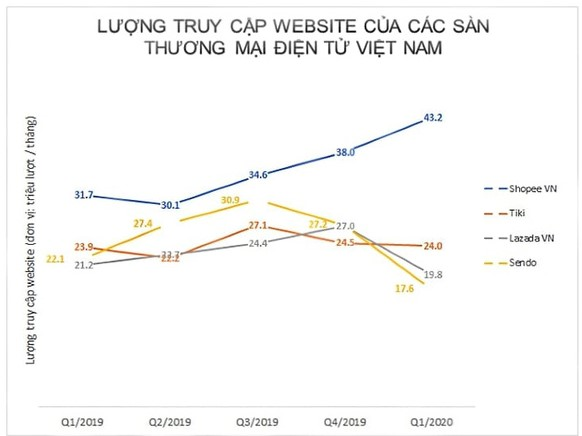
\includegraphics[width=0.5\textwidth]{image/tmdt.JPG}
\caption{\label{fig:tmdt} Lượng truy cập website của các sản thương mại điện tử Việt Nam}
\end{figure}
Bản đồ TMĐT Việt Nam quý I-2020 do website tìm kiếm và so sánh giá iPrice Group cùng công ty đo lường SimilarWeb vừa công bố cho chúng ta cái nhìn cụ thể hơn về vấn đề này.
\begin{itemize}
    \item \textbf{Top sàn TMĐT Việt Nam quý I-2019 có chút ít thay đổi.}  
    
Bốn “ông lớn” TMĐT Việt Nam vẫn là bốn cái tên quen thuộc, nhưng trật tự có chút thay đổi. Xếp thứ nhất vẫn là Shopee, Tiki đã lấy lại vị trí thứ nhì, vị trí thứ ba và thứ tư lần lượt là Lazada và Sendo.

Như vậy, lượng truy cập vào website của các sàn TMĐT, trừ Shopee, trong quý này giảm trung bình 9\% so với cùng kỳ năm 2019.

Theo iPrice Group, một phần nguyên nhân là do trong đợt dịch, các sàn TMĐT tiết chế các hoạt động quảng cáo và khuyến mãi mà thay vào đó, đẩy mạnh livestream và game trên ứng dụng và mạng xã hội. Mục đích là tận dụng lúc người dân ở nhà và có nhiều thời gian ngồi trước màn hình để tăng tương tác, tăng độ gắn kết với khách hàng, đồng thời thử nghiệm tính năng mới.

Bên cạnh đó, còn có một nguyên nhân nữa là nhu cầu mua sắm trực tuyến của người tiêu dùng trong đợt dịch thay đổi liên tục và khó đoán trước.
\item \textbf{* Thương mại điện tử biến đổi vì dịch}

Dữ liệu của iPrice Group cho thấy do ảnh hưởng của dịch Covid-19 mà quý I vừa qua có một số ngành hàng trực tuyến trở nên “nóng sốt”.

Hưởng lợi đầu tiên là ngành hàng chăm sóc và bảo vệ sức khỏe. Trong tháng 2, nhu cầu tìm mua trực tuyến cho các sản phẩm khẩu trang và nước rửa tay khô lần lượt tăng đến 610\% và 680\% so với tháng 1. Sang đến tháng 3, khi người tiêu dùng ở nhà tránh dịch nhiều hơn thì đến lượt ngành bách hóa trực tuyến lên ngôi. Lượng truy cập vào website của Bách hóa xanh quý này nhờ vậy đã tăng 49\% so với quý IV-2019.

Điều đột biến là ở chỗ các ngành này trước nay không phải là tâm điểm của thị trường TMĐT Việt Nam. Điển hình là trong top 50 website TMĐT Việt Nam chỉ có 2 website chuyên doanh hàng tạp hóa là Bách hóa xanh và BigC, ít hơn nhiều so với 10 website ngành hàng di động và 7 website ngành hàng thời trang. Ngược lại, chính các ngành trước đây là “gà đẻ trứng vàng” của TMĐT Việt Nam như thời trang và điện máy thì trong đợt dịch lại bị ảnh hưởng tiêu cực.

Trong 3 tháng đầu năm, các website ngành thời trang trong bản đồ TMĐT Việt Nam bị sụt giảm trung bình 38\% lượng truy cập so với quý trước. Tương tự, lượng truy cập vào các website ngành điện máy trong tháng 2 giảm 17\% so với tháng 1. Sang tháng 3, thị trường xuất hiện nhu cầu mua laptop, webcam, microphone, màn hình… để phục vụ học tập và làm việc tại nhà nên ngành này đã hồi phục lại.

Như vậy, chỉ sau 3 tháng đầu năm, thị trường TMĐT đã trải qua nhiều biến chuyển do ảnh hưởng của Covid-19. Điều này vừa mang đến các cơ hội mới, vừa đặt ra thách thức cho các sàn và các website TMĐT, đòi hỏi họ phải nhanh nhạy và luôn sẵn sàng thay đổi.

Ví dụ như một số website bán hàng mỹ phẩm nay có bán thêm khẩu trang và nước rửa tay khô. Kết quả cho thấy lượng truy cập vào các website này trong quý I-2020 tăng trung bình 32\% so với quý IV-2019. Còn các website thuần bán mỹ phẩm thì chỉ tăng trung bình 10%.

Trong khi đó, bốn sàn TMĐT Việt Nam đến tháng 3 mới bắt đầu tập trung đẩy mạnh các mặt hàng bách hóa, chăm sóc sức khỏe phục vụ đợt dịch, còn trước đó thì vẫn là các ngành hàng thời trang, điện máy, mỹ phẩm chiếm vị trí chủ đạo trên trang chủ và trong các chiến dịch khuyến mãi.

Chỉ sau khi các sàn bắt đầu chuyển dịch mặt hàng theo các nhu cầu mới của thị trường thì đến cuối quý I, lượng truy cập vào website của các sàn mới đồng loạt tăng trở lại, cho thấy những dấu hiệu khởi sắc cho TMĐT thời gian tới đây.
\end{itemize}

\section{An ninh trong thương mại điện tử}
\subsection{Vấn đề}

Làm thế nào để cân bằng giữa an ninh và tiện dụng. Một hệ thống càng an toàn thì khả năng xử lý, thực thi thao tác càng phức tạp.

\begin{itemize}
    \item Các loại tội phạm trong e-commerce rất tinh vi trong khi việc giảm các rủi ro thương mại điện tử là một quá trình phức tạp liên quan đến những đạo luật mới, công nghệ mới, nhiều thủ tục và các chính sách tổ chức. E-commerce đã hấp dẫn các tin tặc khi khách hàng sử dụng thẻ để mua hàng hoặc dịch vụ trực tuyến, dùng email để thực hiện các giao dịch kinh tế.
    \item  Các yếu tố làm số lượng các tấn công trên mạng phát triển.
    \begin{itemize}
        \item - Các hệ thống an ninh luôn tồn tại các điểm yếu. 
        \item - Vấn đề an ninh và dễ dàng sử dụng.
        \item - Vấn đề an ninh thường xuất hiện sau khi có sức ép thị trường.
        \item - Vấn đề an ninh của trang e.commerce còn phụ thuộc vào an ninh của internet, số lượng các trang web của các trường, thư viện, cá nhân…
    \end{itemize}
\end{itemize}
\subsection{An ninh thương mại điện tử}
\subsubsection{Những quan tâm về vấn đề an ninh thương mại điện tử}
\begin{itemize}
    \item \textbf{Phía người mua: Bằng cách nào ?}
    
      - Biết chắc Website do một công ty hợp pháp quản lý và sở hữu
      .
      - Biết chắc trang web không chứa các đoạn mã nguy hiểm hoặc các nội dung không lành mạnh.
      
      -  Biết chắc rằng web server sẽ không cung cấp các thông tin của người sử dụng cho một người khác.
      
    \item \textbf{Phía người bán: Bằng cách nào ?}
    
      - Người sử dụng sẽ không xâm nhập vào trang web để thay đổi các trang và nội dung trên đó. 

      - Người sử dụng sẽ không phá hoại website để những người khác không thể sử dụng được. 
      
     \item \textbf{Từ phía cả công ty và người sử dụng: bằng cách nào họ có thể biết chắc rằng}
     
     -  Đường truyền sẽ không bị người thứ ba theo dõi. 
     
     -  Các thông tin được lưu chuyển giữa hai bên sẽ không bị thay đổi.
\end{itemize}
\subsubsection{Các khía cạnh của an ninh thương mại điện tử}
Hoạt động thương mại điện tử cần đảm bảo các yếu tố sau:
\begin{itemize}
    \item Tính toàn vẹn.
    \item Chống phủ định
    \item Tính xác thực
    \item Tính đáng tin cậy
    \item Tính riêng tư
\end{itemize}
\subsubsection{Những nguy cơ đe dọa an ninh thương mại điện tử}
Những nguy cơ đe dọa là:
\begin{itemize}
\item Các đoạn mã nguy hiểm (malicious code): gồm nhiều mối đe dọa khác nhau như các loại virus, worm.

\item Tin tặc (hacker) và các chương trình phá hoại (cybervandalism)

\item Gian lận thẻ tín dụng

\item Sự lừa đảo: Tin tặc sử dụng các địa chỉ thư điện tử giả
hoặc mạo danh một người nào đó nhằm thực hiện
những hành động phi pháp.

\item Sự khước từ dịch vụ: là việc các hacker sử dụng những giao thông vô ích làm tràn ngập hoặc tắc nghẽn mạng truyền thông, hoặc sử dụng số lượng lớn máy tính tấn công vào một mạng.

\item Nghe trộm, giám sát sự di chuyển của thông tin trên mạng. Xem lén thư điện tử là sử dụng các đoạn mã ẩn bí mật gắn vào một thông điệp thư điện tử, cho phép người xem lén có thể giám sát toàn bộ các thông điệp chuyển tiếp được gửi đi với thông điệp ban đầu.
\end{itemize}

\subsubsection{Một số giải pháp công nghệ đảm bảo an ninh thương mại điện tử}
Kỹ thuật mã hóa thông tin: là quá trình chuyển các văn bản hay các tài liệu gốc thành các văn bản dưới dạng mật mã để bất cứ ai, ngoài người gửi và người nhận đều không thể đọc được.
 
\textbf{Hệ thống mã hóa hiện đại thường được số hóa} – thuật toán dựa trên các bit đơn của thông điệp chứ không dựa trên ký hiệu chữ cái. Máy tính lưu trữ dữ liệu dưới dạng một chuỗi nhị phân, trình tự của các số 1 và 0. Mỗi ký tự gọi là một bit. Các mã khóa và mã mở là các chuỗi nhị phân với độ dài khóa được xác định sẵn.
 
Ngày nay, hai kỹ thuật cơ bản thường được sử dụng để mã hóa thông tin trên internet là mã hóa “khóa riêng” hay mã hóa “khóa bí mật” và mã hóa “khóa công cộng”. 

\begin{itemize}
    \item Mã hóa “khóa bí mật” còn gọi là mã hóa đối xứng, người gửi mã khóa một thông điệp sử dụng khóa bí mật đối xứng, sau đó gửi thông điệp đã mã hóa và bí mật đối xứng cho người nhận bằng một cách nào đó mà họ cảm thấy là an toàn. 
    \item Mã hóa công cộng: là phương pháp sử dụng hai mã khóa cho quá trình mã hóa, một mã dùng để mã hóa thông điệp, một mã để giải mã thông điệp. Mỗi người sử dụng có hai loại mã khóa: mã khóa bí mật chỉ riêng người đó biết, còn mã khóa công cộng được thông báo rộng rãi cho những người sử dụng khác trong hệ thống. Người gửi sử dụng mã khóa công cộng của người nhận để mã hóa thông điệp. Người nhận khi nhận được thông điệp sẽ sử dụng mã khóa cá nhân của mình để giải mã thông điệp.
\end{itemize}

\textbf{Giao thức thỏa thuận mã khóa:} Một trong những giao thức thỏa thuận mã khóa là phong bì số hóa. Thông điệp được mã hóa bằng mã khóa bí mật và sau đó mã khóa bí mật được mã hóa bằng mã khóa công cộng. Người gửi sẽ gửi kèm thông điệp đã được mã hóa (bằng khóa bí mật) và khóa bí mật được mã hóa (bằng khóa công cộng) và gửi toàn bộ cho người nhận.

\textbf{Chữ ký điện tử: }Là một biện pháp mã khóa công cộng được sử dụng phổ biến trong e.commerce, đó là bất cứ âm thanh điện tử, ký hiệu hay quá trình điện tử gắn với hoặc liên quan một cách logic với một văn bản điện tử khác theo một nguyên tắc nhất định và được người ký (hay có ý định ký) văn bản đó thực thi hoặc áp dụng. - Chứng thực điện tử: là trung tâm an ninh trong TMĐT, thông qua bên thứ 3, là công cụ dễ dàng và thuận tiện để các bên tham gia giao dịch tmđt tin tưởng lẫn nhau.

\textbf{An ninh mạng và bức tường lửa:}

\begin{itemize}
    \item Mục tiêu của an ninh mạng là chỉ cho phép người sử dụng được cấp phép truy cập thông tin và dịch vụ.
    \item Bức tường lửa: bảo vệ mạng LAN khỏi những người xâm nhập từ bên ngoài. Mỗi mạng LAN có thể kết nối với internet qua một cổng và thông thường phải có tường lửa.
    \begin{itemize}
        \item Các loại tường lửa:
        \begin{itemize}
            \item Tường lửa lọc gói
            \item Cổng ứng dụng
            \item Cổng mức mạch
        \end{itemize}

    \item Lựa chọn tường lửa:
        \begin{itemize}
            \item Cấu hình tường lửa là sự áp dụng chính sách an ninh thông tin cho mạng máy tính.
            \item Triển khai tường lửa tùy thuộc vào yêu cầu an ninh của tổ chức hay DN và khả năng tài chính của DN đó
        \end{itemize}  
    \end{itemize}
\end{itemize}

\section{Kết luận}

Thương mại điện tử đang phát triển mạnh mẽ, là một phần không thể thiếu trong hoạt động của doanh nghiệp trên toàn thế giới. Quy mô thị trường thương mại điện tử của Việt Nam với xuất phát điểm khá khiêm tốn, khoảng 4 tỷ USD vào năm 2015, nhưng tăng trưởng khá nhanh và ổn định trong những năm 2016, 2017, 2018, nếu tiếp tục giữ mức tăng trưởng 30\%/năm thì thị trường ước tính đạt 13 tỷ USD vào năm 2020. Với tốc độ tăng trưởng nhanh và ổn định như vậy, kết hợp với xu hướng chuyển dịch thói quen mua sắm của người tiêu dùng, có thể khẳng định thương mại điện tử sẽ ngày càng chiếm lĩnh những vị thế quan trọng hơn đối với các doanh nghiệp. Bài viết khái quát những lợi ích của doanh nghiệp khi tham gia thị trường thương mại điện tử và những xu hướng nổi bật của các doanh nghiệp khi phát triển mô hình thương mại điện tử hiện nay.

Hoạt động thương mại điện tử tại Việt Nam vẫn trong giai đoạn đầu phát triển, mới chỉ ứng dụng mạnh mẽ trong vòng 4 năm trở lại đây. Tuy nhiên, nước ta cũng đã triển khai được một số ứng dụng thương mại điện tử như trong mua bán hàng hóa dịch vụ, cung cấp dịch vụ công cho dù kết quả đạt được chưa cao. Các hoạt động thương mại điện tử đã triển khai tại Việt Nam chỉ mới mang tính hình thức do hạn chế về hạ tầng kỹ thuật cũng như nhận thức của người dân.  

Tiềm năng tăng trưởng: Theo các chuyên gia kinh tế, Việt Nam hiện đang có nền tảng vững chắc để phát triển thương mại điện tử. Thống kê cho thấy, Việt Nam nằm trong số 78\% các quốc gia trên thế giới có giao dịch điện tử và nằm trong số 38\% quốc gia có chính sách bảo vệ người tiêu dùng; 45\% quốc gia có chính sách bảo vệ dữ liệu cá nhân và trong số 75\% quốc gia có Luật An ninh mạng…

Việt Nam cũng có hơn 64 triệu người sử dụng internet, 57\% dân số có tài khoản mạng xã hội, 67\% người dùng internet đã từng mua hàng trực tuyến ít nhất 1 lần... Đặc biệt, Chính phủ Việt Nam rất quan tâm đến việc ứng dụng các thành tựu của cuộc Cách mạng công nghiệp 4.0 bằng việc đã ban hành nhiều cơ chế, chính sách cho thương mại điện tử phát triển nhanh, bền vững trong vài năm tới.

Theo Báo cáo Chỉ số thương mại điện tử năm 2019 của Hiệp hội Thương mại điện tử Việt Nam (VECOM), nếu tốc độ tăng trưởng của năm 2019 và 2020 tiếp tục ở mức 30\% thì tới năm 2020 quy mô thương mại điện tử bán lẻ sẽ lên tới 13 tỷ USD, cao hơn so với mục tiêu nêu trong Kế hoạch tổng thể phát triển thương mại điện tử giai đoạn 2016-2020 (đạt 10 tỷ USD vào năm 2020).

Trong khi đó, theo nhận định của Tổng cục Thống kê, dự kiến, doanh thu bán lẻ thương mại điện tử đến năm 2020 còn khả quan hơn, với khoảng 13-15 tỷ USD. Trước đó, Công ty Nielsen Việt Nam cũng dự báo, với sự tăng trưởng lên tới 22\%/năm, quy mô thị trường thương mại điện tử Việt Nam có thể đạt mức 10 tỷ USD đến cuối năm 2020. Trong khi, nghiên cứu của Google và Quỹ đầu tư Temasek công bố tháng 11/2018 khẳng định, đến năm 2025, tốc độ tăng trưởng của ngành thương mại điện tử Việt Nam lên tới 43\%, cao nhất trong các nước Đông Nam Á.

\end{document}